\usepackage{amsmath}
\usepackage{unicode-math}
\usepackage{tabto}
\usepackage{graphicx}
\usepackage{float}
\usepackage[section]{placeins}
\usepackage{subfig}

\begin{document}



\maketitle
\thispagestyle{empty}
\pagestyle{empty}


%%%%%%%%%%%%%%%%%%%%%%%%%%%%%%%%%%%%%%%%%%%%%%%%%%%%%%%%%%%%%%%%%%%%%%%%%%%%%%%%
\begin{abstract}

Shape formation by multi-robotic systems has a significant role in research of swarm robotics. Our research relies mainly on using an autonomous decentralized multi-robotic system to achieve shape formation using discrete and continuous algorithms. Our study mainly focuses on the run times and efficiency of the controllers used in decentralized shape formation. Our research uses a consensus algorithm as a basis to relate differences in total distance traveled and time elapsed.

\end{abstract}


%%%%%%%%%%%%%%%%%%%%%%%%%%%%%%%%%%%%%%%%%%%%%%%%%%%%%%%%%%%%%%%%%%%%%%%%%%%%%%%%
\section{INTRODUCTION}

Swarm robotics is a field in which multiple robots (agents) are controlled in a decentralized manner. There are certain requirements to full fill in order for a multi-robotic system to be considered a swarm robotic system. Robots within the multi-robotic system must work autonomously using their basic sensors to interact with the environment and other agents. The algorithms and controllers used in the system must operate for a wide range of total agents. The robotic system must also maintain homogeneity with the robots used such that they are similar physically and in sensing capabilities. 
\subsection{Website}
(add link) 
\subsection{Focus and Expectations}
In this paper we explore the usage of  multi-robotic decentralized controllers for the purpose of creating an efficient and dynamic algorithm for shape formation. Using the feedback from the agents in our system allows our controllers to make a movement decision for each of our agents. Our simulation based experiments consists of large quantity of agents in a given map with and without constraints. 


\subsection{Motivation} 

Swarm robotics has a lot of important and fundamental purposes. Starting with the ability to solve problems by breaking them down and solving them by robots with basic capabilities and sensors. Inspired by insects such as ant swarms in which each member of the colony contributes to a certain task and without the use of a central commander. It is really interesting to see how these insects can group up to complete a task. Similarly in swarm robotics we can search areas for an object, build structures, make shape formations and many other tasks. Motivated by the course EECS106B at the University of California Berkeley and by groups of researchers we decided to go with swarm robotics. From the course EECS106B we learned a lot about path planning with object avoidance and how to create trajectories to a desired position. With our decentralized multi-robotic system we had to construct a way such that the agents would not collide with each other or any other obstacle. Throughout the course we worked a lot with optimization problems and controllers that would allow us to manipulate robots to a desired location. We wanted to delve deeper into convex and non convex optimization problems that could be implemented in a much larger scale such as swarm robotics. In lab we used Rapidly-Exploring Random Trees (RRT) to design a robotic path planner in a non-convex space. We were motivated to search for ways of implementing such a planner that could work for swarm robotics and have each robot find its position and follow a path towards their designated location. The motion planners we worked with at the time of designing the RRT planners did not have moving robot in a global setting which creates an additional layer of constraints. 










\subsection{Methods}

We have two primary goals in this project. The first is to implement a simulator for synchronous decentralized swarms which simulates communication as well as robot motion. The second is to extend Wang and Rubinstein's algorithm from [1] to the continuous domain.


\subsection{Problem statement}

The algorithm we implement aims move a decentralized swarm of $n$ identical robots represented by set $A$ from their initial positions to an arbitrary target formation represented by goal coordinates in set $Q$ using collision- and deadlock-free paths. For this paper we assume $|A| = |Q|$.

Each agent $a_{i} \in A$ is modelled as a circle with radius $r$. We assume that each agent has the same clock frequency $f_{clock}$ and velocity $v$. Each agent communicates its position with negligible latency and communication error to all robots within the communication range $R > 2\sqrt{2}r$ at a fixed rate $f_{comm}$. We define $p_{a_{i}}(t)$ as the position of $a_i$ at time $t$. Similarly, $T_{a_{i}}(t)$ is the position assigned to $a_i$ at time $t$.

Deadlock-free paths are defined as those where no two robots are assigned the same target position once all robots are guaranteed to be at their assigned position. This is formally defined below by Equation 1: $ \exists t_{max} > 0 \ \text{ s.t.} \ \forall t > t_{max}, \ \forall a_{i} \in A, p_{a_{i}}(t) = T_{a_{i}}(t) \text{and} \ \forall a_i \neq a_j, T_{a_{i}}(t) \neq T_{a_{j}}(t) $

Collision free paths, as the name suggests, are those in which the robots never collide. This is formally defined below by Equation 2:
$
 \forall t \geq 0, {} \mbox{for any two agents, } a_i \neq a_j , \Vert p_{a_i}(t) - p_{a_j}(t) \Vert \geq 2r $


\begin{table}
\caption{An Example of a Table}
\label{table_example}
\begin{center}
\begin{tabular}{|c||c|}
\hline
One & Two\\
\hline
Three & Four\\
\hline
\end{tabular}
\end{center}
\end{table}


%%%%%%%%%%%%%%%%%%%%%%%%%%%%%%%%%%%%%%%%%%%%%%%%%%%%%%%%%%%%%%%%%%%%%%%%%%%%%%%%
\section{Related Work}

As we designed controllers and algorithms so we noticed a potential for creating such things for multi-robotic systems in which more restrictions and considerations arise. There are multiple ways of forming and replacing the controllers from a single robotic system to a multi-robotic system. One inspiring way in which a group solved this was to use the physical properties of water [2]. We gained inspiration from this as it gave us a better idea of how to decentralize our system without restricting our robots to specific environment. We noticed that a good approach was to group robots so that they have information of the nearby agents as most swarm robotics have access to. This would allow for the agents to pass through narrow and complicated pathways similar to hydrodynamics. 

Path planning is a big concept in robotics as it develops the trajectory in which a robot can take. Inspired by a group who created a decentralized controller to solve the issue of robots crashing with each other and allowing for the maintenance of the communication we formulated a controller similar to theirs [6]. The code implemented in our bots do acquire information from nearby agents without limiting their abilities as the task we are given does not interrupt the bandwidth available.

 Another research project worked on a consensus algorithm for primitive agents connected through a network, in which each robot was considered a probabilistic finite state machine [3]. We used their grouping technique to converge our continuous and discrete algorithm for shape formation. The algorithm used by this group guarantees convergence for any network size and topology. Using some of their work we were able to run tests with hard edge shapes and of complicated initial group constraints. 
 
 One of the groups that inspired this project used RRT path planner to find the solution from an arbitrary point to a goal position for multiple robots in a convex space. The robots in this system avoided obstacles under global inputs[9]. The main work of this paper is to create solutions to non time-reversible projections such as collisions which usually happens in micro robotic swarm systems. We applied some of the algorithms to calculate the configuration space of the convergence.    
 
 


\addtolength{\textheight}{-3cm}   % This command serves to balance the column lengths
                                  % on the last page of the document manually. It shortens
                                  % the textheight of the last page by a suitable amount.
                                  % This command does not take effect until the next page
                                  % so it should come on the page before the last. Make
                                  % sure that you do not shorten the textheight too much.

%%%%%%%%%%%%%%%%%%%%%%%%%%%%%%%%%%%%%%%%%%%%%%%%%%%%%%%%%%%%%%%%%%%%%%%%%%%%%%%%
\section{Methods}

\subsubsection{Implementation of the synchronous decentralized swarm simulator}

(TODO: Shreyas. Look at slide 11 here: https://docs.google.com/presentation/d/1rkwiDesOz-RFXUJch8n0EQfEvaiO2Npk1NASDOzKvVk/edit?fbclid=IwAR3PeC-W-sRx6EjNNgemoFN3UklKrfKgrsSR7ykSej-pZoGGJoMHq6zRMII#slide=id.g7743aff168_2_330 )

\subsubsection{Algorithm}
(TODO: Shreyas)

\section{Results}

\subsection{Experimental Findings}

\subsubsection{Number of agents}
The first experiment we ran was to understand how the size of the swarm affects the performance of the algorithm. We used two metrics to judge the performance: total distance travelled by the robots and time taken to converge. We were confident that time taken and distance travelled would increase as the number of agents increased since more agents would lead to more path-planning, goal assignment and overall computation. However, we noticed an interesting result in [1] where the algorithm's performance suddenly improves (i.e. the total time and total distance decreases) as the number of agents is increased. Specifically, the performance of the algorithm for ~196 agents is far better than the performance for 25 to 169 and 225 to 529 agents. 

We performed the same experiment with our implementation on our simulator, averaging results over 6 trials per swarm size. The results of this experiment are shown in Figure 1. As expected, we see an overall increase in the runtime and distance travelled as the number of robots is increased. We also see the previously mentioned improvement when using five agents. On visualizing these trials on our simulator we noticed some behaviors that might be causing this anomaly. When the number of agents is too high, the number of agents sharing the same goal is larger, causing a large number of 'wait-flags', leading to increased runtime. There is also excess travel when the robots try to swap goals and form clusters of cyclic 'traffic graphs' which are further discussed in Section IV.C. When the number of agents is too small, the performance is good but two or three robots can hardly be called a swarm. The strange behavior of four agents showing a worse performance than five can be explained through certain behaviors identified in the simulations as well. The four agent case specifically demonstrates a strange behavior where two or three agents form a cluster in adjacent squares and alternate between swapping goals and moving back and forth. This behavior accounts for the worse performance, but can actually be controlled by decreasing the probability of swapping goals in the goal manager. Further experimentation is needed to understand the extent to which this parameter can affect performance. 

\begin{figure}%
    \centering
        \subfloat[Convergence time ]{{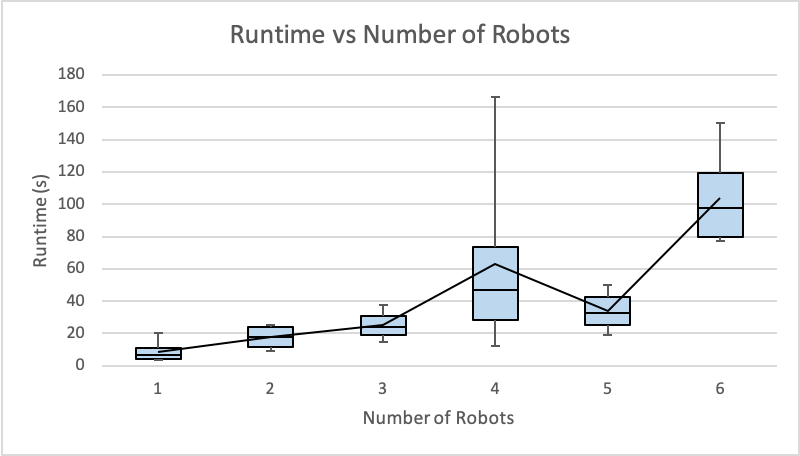
\includegraphics[scale = 0.5]{template/g1_rr.png} }}%
    \qquad
    \subfloat[Total distance travelled]{{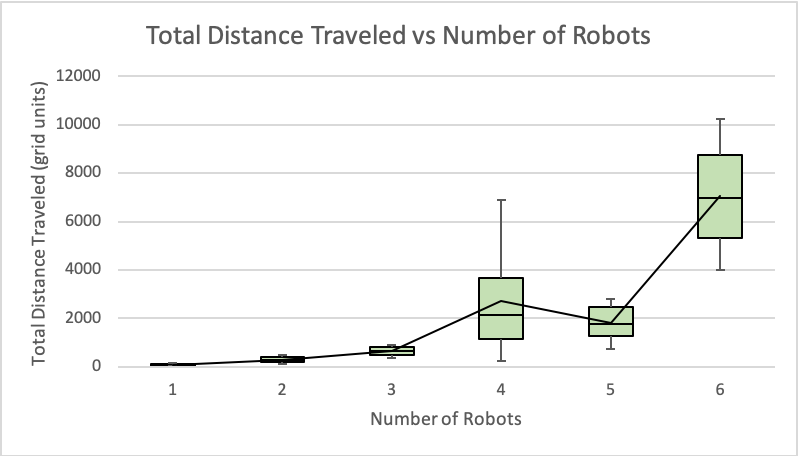
\includegraphics[scale = 0.5]{template/g2_td.png} }}%
    \caption{Results averaged over 36 trials of the discrete version of the algorithm run on our simulator}%
    \label{fig:example}%
\end{figure}

\subsubsection{Continuous vs Discrete}
(TODO: shreyas experiemtns needed) 

\subsection{Safety Guarantees}

In this section we will show that the collision-free and deadlock-free guarantees hold in the continuous case as well using similar arguments as [1]. Let $W_{a_i}(t)$ be the waypoint that is currently assigned to $a_i$. Also define $\Delta t = \frac{2}{f_{comm}}$. Robots are assigned waypoints which are represented by $W_{a_i}(t)$.


For this proof, let's begin by assuming that all agents start at unique positions with unique initial waypoints. We will prove that when some $a_i$ is assigned a new waypoint at time $t^*$, it will be assigned a waypoint that no other agent is currently occupying or moving towards by contradiction. 

From the pseudocode we can show that the following conditions must be met in order to update the waypoint of an agent $a_i$.

\begin{itemize}
    \item Condition 1: $a_i$ does not receive a wait-flag message between $t^* - \Delta t$ and $t^*$.
    \item Condition 2: For all $t \in (\Delta t - t^*, t^*]$,$ W_{a_i}(t) = W^0$. This is because the agent must wait for at least $\Delta t$ time before the waypoint is updated. 
\end{itemize}
\\

\subsubsection{Deadlock-free Path Guarantee}
First we will prove that the paths are deadlock-free as stated in Equation 1. Assume some robot $a_j$ occupies waypoint $W^{1}$ at $t^*$, when $a_i$ is assigned a new $W_{a_i}(t^*) = W^1$ from original waypoint $W^0$. WLOG, we assume $a_j$ has higher priority than $a_i$. We know that $a_j$ was assigned $W^1$ at some time $t^{1j}$. We can analyze this situation using two cases. 
\begin{itemize}
    \item Case 1: $t^{1j} < t^* - \frac{\Delta t}{2}$ 
This situation implies that $a_i$ and $a_j$ share the same waypoint for $t \in [t^* - \frac{\Delta t}{2}, t^*]$. However, by Condition 1, this is not possible. 
\item 
Case 2:  $t^{1j} \in [t^* - \frac{\Delta t}{2}, t^*]$
This means that $a_j$ was assigned some other waypoint before $t$ by Condition 2 but both $a_i$ and $a_j$ decided to choose the same next waypoint in the interval $[t^* - {\Delta t}, t^* - \frac{\Delta t}{2}]$ . If they are both assigned the same waypoint after this time, they have up to $\frac{\Delta t}{2}$ time to let each other know. Condition 1 will therefore prevent this update from happening since $\frac{\Delta t}{2} = \frac{1}{f_{comm}}$. 
\end{itemize}
Therefore, we have shown by induction that Equation 1 will remain satisfied if initial waypoint assignments are unique. 

\subsubsection{Collision-free Path Guarantee}
We can prove the collision-free paths guarantee in a similar way. Let's assume $a_i$ and $a_j$ are moving towards each other in opposite directions at time $t^*$. At the some $t < t*$, assume $W_{a_i}(t) = W^0$ and $W_{a_j}(t) = W^1$. Since the agents move towards each other at time $t^*$, we know that $W_{a_i}(t^*) = W^1$ and $W_{a_j}(t^*) = W^0$. This situation can also be analyzed using two cases. 
\begin{itemize}
    \item Case 1: The time $t_{a_i}^{u} < t$ at which the agents decide to update their waypoints is different. This case is the same as the previously proven deadlock-free guarantee and can never exist. 
\item Case 2: The time at which the new waypoints are determined is the same. This means that the robots share a future waypoint for up to $\frac{\Delta t}{2}$ time, which is enough time for Condition 1 to prevent or delay one of the waypoint updates.
\end{itemize}
\\
Therefore, there cannot be any collisions on these paths.

\subsection{Convergence}

Our implementation of the algorithm in the discrete case guarantee almost sure convergence. The proof from [1] is quite involved and exhaustively analyzes multiple cases to prove the claims being made. This section will provide a higher-level idea of this proof. 

First define two loss functions $J_1(t)$ and $J_2(t)$ that reach 0 when the agents achieve the goal state as follows: 
\begin{itemize}
    \item $J_1(t) = \sum_{i=1}^{|A|} d_i(t) = $ the total distance of each agent to its assigned goal position at time $t$. Here $d_i(t)$ is the Manhattan distance from the agents position to the goal.
    \item $J_2(t) = |Q| -  \sum_{i=1}^{|q|} \mathbb{1}_i(t) $ number of goals that no agent is moving towards  $t$. Here, $\mathbb{1}_i(t)$ is an indicator variable for the event that some agent's target position at time $t$ is goal position $i$.
\end{itemize}
It follows from the definition of these loss functions that the algorithm converges if both of these loss functions converge. 
To show almost sure convergence, we must prove that the loss functions are:
\begin{itemize}
    \item Bounded and non-negative 
    \item Non-increasing
    \item Strictly decreasing with non-zero probability for all values except $J = 0$
\end{itemize}

\subsubsection{Bounded and non-negative} The loss functions are non-negative by definition. They can also be bounded by considering the fact that agents move greedily at each step. This implies that $J_2 \leq |A| - 1$ since at least 1 goal is assigned to the swarm. The total distance from goals also decreases due to this greedy approach, implying that $J_1 \leq k|A|$ where $k$ is the maximum distance between any goal state and any initial position on an agent.

\subsubsection{Non-increasing} As explained in the previous part, $J_2$ is always decreasing as at least one agent moves towards its target position. Once $J_2 = 0$, each agent is assigned to a unique goalstate, and $J_1$ can only decrease as the agents move towards it.

\subsubsection{Strictly decreasing in probability} This part of the proof exhaustively looks at cases to prove the claim. Please refer to Lemma IV-B.4 from [1] for a more detailed explanation of this proof. We can form a 'traffic graph' for some time-step with agents represented by vertices, and edges between nodes $i$ and $j$ if $a_i$ wants to move to a point occupied by $a_j$. Under this formulation, all nodes with zero out-degree are called "head nodes" as their path is not blocked. 
\\ 
There are 3 cases we can consider:
\begin{itemize}
    \item Case 1: If the 'traffic graph' is acylic and there exists some head agent $a_i$ that has not reached it's goal. By definition, this agent has a free path and can reduce $J_{1}$ by 1.
    \item Case 2: If the graph is cyclic. It can be shown by contradiction, that agents will always be able to swap goals in the opposite direction of the cycle without the need to move with non-zero probability. (TODO: refer to random part of psudecode).
    \item Case 3: The graph is acyclic and all head agents have reached a goal. This case can essentially be reduced to one of the above cases by swapping goals with a head agent.
\end{itemize}

This proves almost sure convergence for our algorithm in the discrete case. Note that parts of this proof, such as the definition of $J_1$, rely on the assumption that we're only moving along the edges of our grid-world. Therefore, we cannot make this guarantee for the continuous case. In the (TODO: ref) section, we will discuss ways in which we can modify the algorithm to achieve convergence in the continuous case.








%%%%%%%%%%%%%%%%%%%%%%%%%%%%%%%%%%%%%%%%%%%%%%%%%%%%%%%%%%%%%%%%%%%%%%%%%%%%%%%%
\section{CONCLUSIONS AND FUTURE WORKS}

\subsection{Conclusions}

TODO (from slides) 
\subsection{Future Works}
TODO (from slides)


%%%%%%%%%%%%%%%%%%%%%%%%%%%%%%%%%%%%%%%%%%%%%%%%%%%%%%%%%%%%%%%%%%%%%%%%%%%%%%%%
\section{ACKNOWLEDGMENTS}

The authors gratefully acknowledge the contribution of National Research Organization and reviewers' comments.


%%%%%%%%%%%%%%%%%%%%%%%%%%%%%%%%%%%%%%%%%%%%%%%%%%%%%%%%%%%%%%%%%%%%%%%%%%%%%%%%

\begin{thebibliography}{99}

\bibitem{c1}
H. Wang and M. Rubenstein, "Shape formation in homogeneous swarms using local task swapping," IEEE Transactions on Robotics, pp. 1-16, 2020

\bibitem{c2}
C. A Pimenta L A, S. Pereira G, Kumar V, Chaimowicz L M, Bosque M C, Mesquita R. and Michael N. Swarm Coordination Based On Smoothed Particle Hydrodynamics Technique. [Accessed 10 April 2013].

\bibitem{c3}
Liu, Y., Lee, K. Probabilistic consensus decision making algorithm for artificial swarm of primitive robots. SN Appl. Sci. 2, 95 (2020). https://doi.org/10.1007/s42452-019-1845-x 

\bibitem{c4}
V. J. Lumelsky, Continous Robot Motion Planning In Unknown Environment, pp. 339-358. Boston, MA:Springer US, 1986

\bibitem{c5}
G. Li, D. St-Onge, C. Pinciroli, A. Gasparri, E. Garone, and G. Beltrame, "Decentralized progressive shape formation with robot swarms," Auton. Robots, vol. 43, no. 6,pp. 1505-1521, 2019.

\bibitem{c6}
 
Hsieh, Mong-Ying A., Vijay Kumar and Luiz Chaimowicz. (2008). Decentralized controllers for shape generation
with robotic swarms. Robotica. Vol 26(5). p.691-701.

\bibitem{c7}
P. Ghassemi and S. Chowdhury, "Decentralized informative path planning with exploration-exploitation balance for swarm robotic search," ArXiv, vol

\bibitem{c8}
I. Navarro and F. Matia, "An introduction to swarm robotics," ISRN Robotics, vol. 2013, 09 2012.

\bibitem{c9}
Joshi, P., Leclerc, J., Bao, D. and T. Becker, A., 2020. Motion-Planning Using Rrts For A Swarm Of Robots Controlled By Global Inputs. [ebook] Available at: <https://swarmcontrol.ece.uh.edu/wp-content/papercite-data/pdf/8842916.pdf> [Accessed 15 May 2020].
\end{thebibliography}

\end{document}
